\documentclass[11pt]{article}
\usepackage{bookmark}
\usepackage[utf8]{inputenc}
\usepackage{authblk}
\usepackage{amsmath,amsfonts,amsthm,amssymb,mathtools}
\usepackage[english]{babel}

%% theorem, lemma, proof, etc. %%
%% for unnumbed use \newtheorem* and delete section in [---] %%
\newtheorem{theorem}{Theorem}[section]
\newtheorem{corollary}{Corollary}[theorem]
\newtheorem{lemma}[theorem]{Lemma}
\newtheorem{proposition}[theorem]{Proposition}

\theoremstyle{remark}
\newtheorem{remark}{Remark}

\theoremstyle{definition}
\newtheorem{definition}{Definition}[section]

\theoremstyle{definition}
\newtheorem{example}{Example}[section]
%%% theorem %%

\usepackage{enumitem}
\usepackage{graphicx}
\usepackage{tikz}
\usetikzlibrary{decorations.fractals}
\usepackage{float}
\usepackage{dsfont}
\usepackage{geometry}
\geometry{
    a4paper,
    left=30mm,
    right=30mm,
    top=20mm,
    bottom=20mm,
}

%%%% hyperref %%%%
\usepackage{hyperref} % for link
\hypersetup{
    colorlinks=true,
    allcolors=black,
}
%%% fancyhdr %%%% for footer and Hader of document
\usepackage{fancyhdr}
%\pagestyle{fancy}
%\lhead{lest hand head} %% left Hader %%
%\rhead{Measure Theory} %% right Hader %%
\cfoot{\thepage} %% central footer %%

\setlength{\headheight}{14.49998pt}

%%% spacing in document %%%
\usepackage{setspace}
\onehalfspacing

\begin{document}
\begin{titlepage}
    \begin{center}
        \Huge{\textbf{Measure Theory}}

        \vspace{5cm}

        \Large\textbf{{
                Name: AZMAIN BISWAS\\
                Roll No.: 2022MAM008\\
                Supervisor's Name: Dr. UJJAL DEBNATH\\
                Mini Project for 1st semester course in\\
                M.Sc. in Applied Mathematics}}

        \vspace{2cm}

        
\includegraphics[scale = 0.4]{pic/iiest.png}

        \vspace{2cm}

        \Large\textbf{{
                Department of Mathematics\\
                INDIAN INSTITUE OF ENGINEERING SCIENCE AND TECHNOLOGY, Shibpur}}

                \vspace{3cm}

        \large{DECLARATION: I affirm that I have identified all my sources and that no part of my dissertation paper uses unacknowledged materials.}
    \end{center}
\end{titlepage}

\newpage
\newcommand{\tx}[1]{\text{#1}}
\newcommand{\smu}{\mu^{*}}
\newcommand{\tld}[1]{\tilde{#1}}
\newcommand{\sig}{$\sigma$}
\newcommand{\RR}{$\mathds{R}$}
\newcommand{\A}{$\mathcal{A} $}
\newcommand{\XX}{$X$}
\newcommand{\B}{$\mathcal{B}$}
\newcommand{\F}{$\mathcal{F} $}
\newcommand{\BS}{$\mathcal{B}^*$}
\begin{center}
    \LARGE{\textbf{ACKNOWLEDGEMENT}}
\end{center}
\begin{flushleft}
    \large
    I would like to take this opportunity to express my profound gratitude to my supervisor Dr. Ujjal Debnath 
    for his exemplary guidance and constant encouragement throughout the course of this project. 

    \vspace{5mm}
    I am grateful to IIEST, Shibpur for providing me with the opportunity to complete my dissertation. 
    In this project I have tried to give a short overview of \textbf{Measure Theory}.

    \vspace{5mm}
    I would like to extend my deepest gratitude and thanks to my parents without whose constant support and encouragement this project would never have been completed. 
    I would also like to thank my friends for their valuable suggestions and support.
\end{flushleft}

\begin{flushright}
    \large
    Azmain Biswas
\end{flushright}

\begin{center}
    \LARGE{\textbf{Abstract}}
\end{center}

Measure Theory is the study of Measure. Here we try extend the notion of size of interval to more general sets. We know the size of a interval in $\mathds{R}$ is 
its length. Then by instinct we say in $\mathds{R}^{2}$ it will be area and in $\mathds{R}^{3}$ it will be volume of sets. Finding more general notion of size of
interval leads us to concept of measure.

We will start with outer measure even though it looks promising but it fails to have crucial property. This unfortunate result leads us to \sig-algebra and measurable space. From there we construct measure in an abstract context. Taking restriction on outer measure we construct Lebesgue Measure
which leads to more general theory of integration then Riemann integration.

\tableofcontents
\section{Outer Measure}
\begin{definition}[length of open interval]
    The length $\ell(I)$ of an open interval is define by
    $$
    \ell(I)=
     \begin{cases}
         b-a \ \ &\text{if}\ I=(a-b) \text{for some}\ a,b\in\mathds{R}\ \text{with}\ a<b,\\
         0 \ \ &\text{if}\ I=\emptyset,\\
         \infty\ \ &\tx{if}\ I=(-\infty,a) \ \tx{or}\ I=(a,\infty)\ \tx{for some}\ a\in\mathds{R}\\
         \infty\ \ &\tx{if}\ I=(-\infty,\infty).
    \end{cases}
    $$
\end{definition}

\begin{definition}[Outer Measure]
    The outer measure $\smu(A)$ of a set  $A\subset \mathds{R}$ is define by
    \[
        \smu(A)=\inf \left\{ \sum_{k=1}^{\infty}\ell(I_k) \right\} 
    \]
    where, $I_1,I_2,\ldots$ are open intervals such that $A\subset\cup_{k=1}^{\infty}I_k$.
\end{definition}
\begin{example}[finite sets have outer measure $0$]
    Suppose $A=\{ a_1,a_2,\ldots,a_n \} $ is a finite set of real numbers. Suppose $\epsilon>0$. Define a sequence  $I_1,I_1,\ldots$ of open intervals
    by
    \[
        I_k=
        \begin{cases}
            (a_k-\epsilon,a_k+\epsilon)\ \ \ &\tx{if}\ k\le n;\\
            \emptyset \ &\tx{if}\ k>n.
        \end{cases}
    \]
    Then $I_1,I_2,\ldots$ is a sequence of open intervals whose union contain $A$. \\
    Clearly,  $\sum_{k=1}^{\infty}\ell(I_k)=2\epsilon n$.\\
    Hence, $\smu(A)\le 2\epsilon n$.\\
    Since $\epsilon$ is arbitrary small positive number,  $\smu(A)=0$.
\end{example}

%%%%%%%%%%%%%%%%%%%%%
\subsection{Properties of Outer Measure}
Properties of outer measure are followings,
\begin{enumerate}
    \item Every countable subset of $\mathds{R}$ has outer measure $0$.
    \item Suppose  $A$ and  $B$ are subset of  $\mathds{R}$ with $A\subset B$. Then  $\smu(A)\le \smu(B)$.
    \item Suppose $t\in\mathds{R}$ and $A\subset \mathds{R}$. Then $\smu(t+A)=\smu(A)$.
    \item Suppose  $A_k$'s are a sequence of subset of  $\mathds{R}$. Then,
        \[
            \smu\left( \bigcup_{k=1}^{\infty}A_k \right)\le \sum_{k=1}^{\infty}\smu(A_k). 
        \]
    \item Suppose $a,b\in\mathds{R}$, with $a<b$. Then  $\smu([a,b])=b-a$.
\end{enumerate}
\begin{theorem}[outer measure is note additive]
    \label{nonadditivity OM}
    There exist disjoint subsets $A$ and  $B$ of  $\mathds{R}$ such that,
    \[
        \smu(A\cup B)\neq \smu(A)+\smu(B).
    \]
\end{theorem}
\begin{proof}
    For $a\in[-1,1]$, let  $\tilde{a}$ be the set of numbers in  $[-1,1]$ such that.
     \[
         \tilde{a}=\{c\in[-1,1]:a-c\in\mathds{Q}\}.
    \]
    If $a,b\in[-1,1]$ and  $\tld{a}\cap\tld{b}\neq \emptyset$, Then $\tld{a}=\tld{b}$.\\
    (\textit{Proof: } Suppose There exist $d\in\tld{a}\cap\tld{b}$. Then  $a-b$ and  $b-d$ are rational number; subtracting, we conclude that 
    $a-d$ is rational number. The equitation $a-c=(a-b)+(b-c)$ now implies that if  $c\in[-1,1]$, then $a-c$ is rational iff $b-c$ is rational number.
    In other word  $\tld{a}=\tld{b}$.)\\
    Clearly, $a\in\tld{a}$ for each  $a\in[-1,1]$. Thus $[-1,1]=\cup_{a\in[-1,1]}\tld{a}$.\\
    Let $V$ be a set that contains exactly one element in each of the distinct sets in  $\{\tld{a}:a\in[-1,1]\}$

    In other words, for every  $a\in[-1,1]$, the set  $V\cap\tld{a}$ has exactly one element.

    Let  $r_1,r_2,\ldots$ be a sequence of distinct rational numbers such that
    \[
        [-2,2]\cap\mathds{Q}={r_1,r_2,\ldots}
    \]
    Then
    \[
        [-1,1]\subset \bigcup_{k=1}^{\infty}(r_k+V),
    \]
    Where the set inclusion above holds because if $a\in[-1,1]$ then  $v$ is the unique element of  $V\cap\tld{a}$, we have $a-v\in\mathds{Q}$, which implies that $a=r_k+v\in r_k+V$ for some  $k\in\mathds{Z}^{+}$.

    Then by order-preserving property of outer measure, and countable subadditivity of outer measure imply
    \[
        \smu([-1,1])\le \sum_{k=1}^{\infty}\smu(r_k+V).
    \]
    Now $\smu([-1,1])=2$ and by translation invariance property of outer measure we can say,
     \[
         2\le \sum_{k=1}^{\infty}\smu(V).
    \]
    Thus $\smu(V)>0$.

    Note that the sets  $r_k+V$'s are disjoint.\\
    (\textit{Proof:} Suppose there exists $t\in(r_j+V)\cap(r_k+V)$. Then $t=r_j+v_1=r_k+v_2$ for some  $v_1,v_2\in V$, which implies that  $v_1-v_2=r_k-r_j\in\mathds{Q}$ from the construction of $V$ now implies that  $v_1=v_2\implies r_j=r_k\implies j=k$. ) 
    Let $n\in\mathds{Z}^{+}$. Clearly,
    \[
        \bigcup_{k=1}^{n}(r_k+V)\subset [-3,3]
    \]
    Because $V\subset [-1,1]$ and each  $r_k\in[-2,2]$. The set inclusion above implies that
     \begin{equation}
         \label{less6}
         \smu\left(\bigcup_{k=1}^{n}(r_k+V)\right)\le 6 
    \end{equation}
    However,
    \begin{equation}
        \label{nV}
        \sum_{k=1}^{n}\smu(r_k+V)=\sum_{k=1}^{n}\smu{V}=n\smu(V).
    \end{equation}
    Now (\refeq{less6}) and  (\refeq{nV}) suggest that we choose $n\in\mathds{Z}^{+}$ such that $n\smu(V)>6$. Thus,
     \begin{equation}
        \label{contra}
         \smu\left( \bigcup_{k=1}^{n}(r_k+V) \right) <\sum_{k=1}^{n}\smu(r_k+V).
    \end{equation}

    If we had $\smu(A\cup B)=\smu(A)+\smu(B)$ for all disjoint subset  $A,B$ of  $\mathds{R}$, then by induction on $n$ we would have $\smu\left(\bigcup_{k=1}^nA_k\right)=\sum_{k=1}^n\smu(r_k+V)$. For all disjoint subset $A_1,A_2,\dots,A_n$ of $\mathds{R}$.

    However, from (\refeq{contra}) we see no such result holds. Thus, there exist disjoint subsets on $A,B$ of $\mathds{R}$ such that $\smu(A\cup B)\neq\smu(A)+\sum(B)$. 
\end{proof}

Now we have seen in above theory that outer measure is not additive. So does there exist other notion than outer measure for size of subsets of $\mathds{R}$ that follow additive property?
\begin{theorem}[nonexistence of extension of length to all subset of $\mathds{R}$]
    \label{no length for all set}
    There does note exist a function $\mu$ with all the following properties:
    \begin{enumerate}
        \item $\mu:P(\mathds{R})\to [0,\infty]$.
        \item $\mu(I)=\ell(I)$ for every open interval $I\subset \mathds{R}$.
        \item $\mu\left(\bigcup_{k=1}^{\infty}A_K\right)=\sum_{k=1}^{\infty}\mu(A_k)$ for every disjoint sequence $\{A_k\}$ of subsets of $\mathds{R}$.
        \item $\mu(t+A)=\mu(A)$ for  every $A\subset \mathds{R}$ and for every $t\in \mathds{R}$.
    \end{enumerate}
\end{theorem}
\begin{proof}
    Suppose there exist a function $\mu$ that follow all the property listed above.

    Observed that $\mu(\emptyset)=0$, as follows from (2) because the empty set is a open interval with length 0.

    If $A\subset B\subset \mathds{R}$, then $\mu(A)\le \mu(B)$, as follows from (3) because we can write $B$ as the union of the disjoint sequence $A,B\setminus A,\emptyset,\emptyset,\ldots$;\\
    Thus,
    \[
    \mu(B)=\mu(A)+\mu(B\setminus A)+0+0+\ldots=\mu(A)+\mu(B\setminus A)\ge \mu(A).
    \]
    If $a,b\in \mathds{R}$ with $a<b$, then $(a,b)\subset [a,b]\subset (a-\epsilon,b+\epsilon)$for every $\epsilon>0$. Thus $b-a\le \mu([a,b])\le b-a+2\epsilon$ for every $\epsilon>0$.
    Hence $\mu([a,b])=b-a$.

    If ${A_k}$ is sequence of subset of $\mathds{R}$, then $A_1,A_2\setminus A_1,A_3\setminus (A_1\cup A_2),\ldots$ is a disjoint sequence of $\mathds{R}$ whose union is $\cup_{k=1}^{\infty}A_k$. Thus,
    \begin{align*}
        \mu\left(\bigcup_{k=1}^{\infty}A_k\right)&=\mu(A_1\cup(A_2\setminus A_1)\cup(A_3\setminus (A_1\cup A_2))\cup\ldots)\\
        &=\mu(A_1)+\mu(A_2\setminus A_1)+\mu(A_3\setminus (A_1\cup A_2))+\ldots\\
        &\le\sum_{k=1}{\infty}(A_k),
    \end{align*}

    We have shown that $\mu$ has all the properties of outer measure  that were used in the proof of (\ref{nonadditivity OM}). Repeating the proof of \ref{nonadditivity OM}, we see that there exist disjoint subset $A,B$ of $\mathds{R}$ such that $\mu(A\cup B)\neq\mu(A)+\mu(B)$. Which is a contradiction of (3). This contradiction completes the proof.
\end{proof}
So the above result shows us we have to give up one of the described properties in our goal of extending the notion of size from intervals to more general sets. 
We can not give up property (2) because the size of an interval needs to be its length. We cannot give up property (3) because additivity is needed. We can not give up (4) either because length have to be translation invariant.


So we are force to relax the property (1) that is, size is not defined for all subset of $\mathds{R}$ 

%%%%%%%%%%%%%%%%%%%%%%%%%%%%%%%%
\section{Measurable Space}
\begin{definition}[\sig-algebra]
    Suppose $X$ is a non empty set and $\mathcal{A}$ is a set of subset of $X$. Then $\mathcal{A}$ is called  \sig-algebra
    on $X$ if the following three condition are satisfied:
    \begin{enumerate}
        \item $\emptyset\in\mathcal{A}$,
        \item if $E\in\mathcal{A}$, than $E^c\in \mathcal{A}$. \textit{(close under complementation)}
        \item if $\{E_k\}$ is a sequence of element of $\mathcal{A},$ then $\bigcup_{k=1}^\infty E_k\in\mathcal{A}$. \textit{(closed under countable union)}
    \end{enumerate}
\end{definition}
\begin{theorem}
    Suppose \A\ is a \sig-algebra on a set \XX. Then 
    \begin{enumerate}
        \item $X\in\mathcal{A}$
        \item If $\{E_k\}$ is a sequence of element of \A, then $\bigcap_{k=1}^\infty\in\mathcal{A}$. \textit{(closed under countable intersection)}
    \end{enumerate}
\end{theorem}
\begin{proof}
    Because $\emptyset \in \mathcal{A}$ and \A\ is closed under complementation so, $X\in\mathcal{A}$.\\
    Now, $E_1,E_2,\ldots$ is in \A\\ 
    then, $E_k^c\in$ \A\ for all $k=1,2,\ldots$.\\
    Then, 
    \begin{align*}
        &\bigcup_{k=1}^\infty E_k^c\in \mathcal{A}.\\
        \implies &\left(\bigcap_{k=1}^\infty E_k\right)^c \in \mathcal{A}\\
        \implies &\bigcap_{k=1}^\infty E_k\in \mathcal{A}.
    \end{align*}
    This proves the result.
\end{proof}

\begin{definition}[measurable space]
    A measurable space is an ordered pair  $(X,\mathcal{A})$, where \XX\ is a set and \A\ is a \sig-algebra on \XX.
\end{definition}

\begin{definition}[measurable set]
    An element of \A\ is called an \A-measurable set or just measurable set.
\end{definition}

%%%%%%%%%%%%%%%%%%%%%%%%%%%%%%%%%%%%%%%%%
\section{Topology Space}

\begin{definition}[Topology]
    A collection $\tau$ of subsets of non-empty set \XX\ is said to be topology in \XX\ if $\tau$ satisfied the following conditions
    \begin{enumerate}
        \item $\emptyset \in \tau \text{ and }X\in \tau$.
        \item if $V_i\in\tau$  for all $i=1,2,\ldots,n$, then $\bigcap_{n=1}^n V_n\in\tau$.
        \item if $\{V_\alpha\}$ is an arbitrary collection of members of $\tau$ (finite, countable, uncountable), then $\bigcup_\alpha V_\alpha\in \tau$.
    \end{enumerate}
\end{definition}

\begin{definition}[topology space]
    If $\tau$ is a topology in \XX, Then an ordered pair  $(X,\tau)$ is called topology space.
\end{definition}

\begin{definition}[Open set]
    The member of $\tau$ is called Open set in \XX.
\end{definition}

\begin{definition}[close set]
    $E$ is said to be closed  set if  $E^c\in\tau$.
\end{definition}



%%%%%%%%%%%%%%%%%%%%%%%%%%%%%%%%%%%%%%%
\section{Borel set}
\begin{theorem}
    \label{smallest sigma algebra}
    If \F\ is any collection of subsets of \XX, there exists a smallest \sig-algebra \B\ in \XX\ such that $\mathcal{F}\in\mathcal{B}$\\
    This \B\ is sometime called the \sig-algebra generated by \F.
\end{theorem}
\begin{proof}
    Let $\Omega$ be the family \sig-algebras \BS\ in \XX\ which contain \F. Since the collection of all subsets of \XX\ is such \sig-algebra (i.e. $P(X)$ is a \sig-algebra), $\Omega$ is non empty.\\
    Let \B\ is  intersection of all $\mathcal{B}^*\in\Omega$. It is clear that $\mathcal{F}\subset\mathcal{B}$ and \B\ lies in every \sig-algebra in \XX\ which contain \F.\\
    To Complete the proof, we have to show that \B\ is a \sig-algebra.
    
    If $A_n\in\mathcal{B}$ for $n=1,2,\ldots$ and if $\mathcal{B}^*\in \Omega$, then $A_n\in\mathcal{B}^*$ so, $\bigcup_{n=1}^\infty A_n\in \mathcal{B}^*$,
    since \BS\ is a \sig-algebra\\
    Since $\bigcup_{n=1}^\infty A_n\in \mathcal{B}^*$ for every $\mathcal{B}^*\in \Omega$, we conclude that $\bigcup_{n=1}^\infty A_n\in \mathcal{B}$. The other two properties of \sig-algebra are verified in the same manner.
\end{proof}

\begin{definition}[Borel  set]
    Let \XX\  be a topology space. By theorem \ref{smallest sigma algebra} there exist a smallest \sig-algebra \B\ in \XX\ such that every open set in \XX\ belongs to \B.  The member of \B\ is called Borel  sets of \XX.
\end{definition}

\textbf{In particular:} The \sig-algebra on \RR\ containing all open subset of \RR\ is called the collection of Borel subset of \RR. An element of this \sig-algebra is called a \textit{Borel Set}.

\begin{example}
    \
    \begin{itemize}
        \item Every closed subset of \RR\ is a Borel set because every closed set are complement of an open subset of \RR.
        \item Every countable subset of \RR\ is a Borel set because countable sets are closed set.
        \item Every half-open interval $[a,b)$ (where $a,b\in \mathds{R}$) is a Borel sets because 
        \[
        [a,b)=\bigcap_{n=1}^\infty\left(a-\frac{a}{n},b\right).
        \]
        \item All countable union of closed sets and all countable intersection of open set are Borel set. This sets are called $F_\sigma$ and $G_\delta$ respectively.
    \end{itemize}
\end{example}


\section{Measurable Function}
\begin{definition}[Measurable Function]
    Let $\left( X,\mathcal{A} \right) $ and $\left( Y,\mathcal{S} \right) $ be two measurable spaces and a function $f:X \to Y$ is said to be $\mathcal{A}$-measurable function(or just measurable function) provided that  $f^{-1}(V)$ is a measurable set in $X$ for every measurable set $V$  in $Y$.\\
    i.e.
    \[
        f^{-1}(V)\in\mathcal{A} \ \ \  \ \text{for every}\ V\in\mathcal{S}
    \]
\end{definition}
\textbf{In particular:} Suppose $(X,\mathcal{A})$ is a measurable space. A function  $f:X\to\mathds{R}$ is called $\mathcal{A}$-measurable if  $f^{-1}(B)\in\mathcal{A}$ for every Borel set $B\subset \mathds{R}$.

\begin{example}
    \
    \begin{itemize}
        \item If $\mathcal{A}$ is a set of all subset of $X$, then every function from  $X\to\mathds{R}$ is a $\mathcal{A}$-measurable.
        \item If $\mathcal{A}=\{\emptyset , (-\infty,0), [0,\infty),\mathds{R}\}$ (which is a $\sigma$-algebra of  $\mathds{R}$), then constant function \\
            $f:\mathds{R}\to\mathds{R}$ is an $\mathcal{A}$-measurable function.
    \end{itemize}
\end{example}

\begin{definition}[characteristic function]
    Suppose $E$ is a subset of  $X$. The characteristic function of $E$ is a function  $\chi_{E}:X\to\mathds{R}$ define by 
    \begin{equation*}
        \chi_{E}(X)=
        \begin{cases}
            1 \ \ \text{if}\ x\in E \\
            0 \ \ \text{if}\ x\notin E
        \end{cases}
    \end{equation*}
\end{definition}
\textbf{Observation:} Suppose $(X,\mathcal{A})$ is a measurable space,  $E\subset X$, and $B\subset\mathds{R}$. Then,
\[
    \chi_E^{-1}(B)=
    \begin{cases}
        E \ \ &\text{if}\ 0\notin B\ \text{and}\ 1\in B.\\ 
        X\setminus E \ \ &\text{if}\ 0\in B\ \text{and}\ 1\notin B.\\ 
        X \ \ &\text{if}\ 0\in B\ \text{and}\ 1\in B.\\ 
        \emptyset \ \ &\text{if}\ 0\notin B\ \text{and}\ 1\notin B.
    \end{cases}
\]
thus we see that $\chi_E$ is an  $\mathcal{A}$-measurable function iff  $E\in\mathcal{A}$.

\begin{definition}[Simple Function]
    Let $\psi$ be real-valued function defined on  $X$. If the range of  $\psi$ is finite, we say that  $\psi$ is a simple function.
\end{definition}
Suppose the range of $\psi$ consists of the distinct number  $c_1,\ldots,c_n$. Let,
\[
    E_i=\{x:\psi(x)=c_i\}\ \ \ (i=1,\ldots,n)
\]
Then,
\[
    \psi(x)=\sum_{k=1}^{n}c_k\chi_{E_{i}}.
\]
i.e. every simple function is a finite linear combination of characteristic functions. Hence it is clear that $\psi$ is measurable iff the sets  $E_1,\ldots E_n$
are measurable.

It is of interest that every function can be approximated by simple function.
\newpage
\begin{theorem}[Approximation by simple function]
    $f:(X,\mathcal{A})\to\mathds{R}^{+}$ is a non-negative measurable function. Then there exists a sequence of simple function $\{\psi_n\}$ such that.
     \begin{enumerate}
         \item $\psi$ is monotone increasing.
         \item  $\lim\psi_n=f$.
     \end{enumerate}
\end{theorem}
\begin{proof}
    Let $k$ be any integer. We write,
     \[
         E_{p,k}=\left\{ x:\frac{p-1}{2^{k}}\le f(x)\le \frac{p}{2^{k}} \right\} \ \text{where}\ p=1,2,\ldots,2^{2k}.
    \]
    and 
    \[
        E_{0,k}=X\setminus \bigcup_{p=1}^{2^{2k}}E_{p,k}=\left\{ x:f(x)\ge 2^{k} \right\}.
    \]
    Then,
    \[
        E_{p,k}=\left\{ x:f(x)<\frac{p}{2^{k}} \right\}\cap\left\{ x:f(x)\ge \frac{p-1}{2^{k}} \right\}.
    \]
    is measurable, Since $f$ is measurable.
    Also, $E_{p,k},\ p=0,1,2,\ldots,2^{2k}$ are mutually disjoint.\\
    we construct,
    \[
        \psi_k(x)=
        \begin{cases}
            \frac{p-1}{2^{k}}\ \ &\text{for} \ x\in E_{p,k}\\
            2^{k} &\text{for} \ x\in E_{0,p}.
        \end{cases}
    \]
    the $\psi_k$ is a step function.\\
    By construction $0\le \psi_k\le f$.\\
    If $x\in E_{p,k},\ p\neq 0$ then we have the following cases.
    
    \textit{Case:1}\\
    $x\in E_{2p-1,k+1}$ in that cases  $\psi_k(x)=\psi_{k+1}$
    
    \textit{Case:2}\\
    $x\in E_{2p,k+1}$ is that case $\psi_k(x)+\frac{1}{2^{k+1}}=\psi_{k+1}(x)$.\\
    Thus for $x\in E_{p,k}$.  Then $\psi_n(x)\le \psi_{n+1}(x)$.\\
    Also, if $x\in E_{0,p}$. Then $\psi_k(x)=2^{k}\le 2^{k+1}=\psi_{k+1}(x)$.
    Combining we get,
    \[
        \psi_k(x)\le \psi_{k+1}(x) \ \ \forall\ x\in X
    \]
    i.e. $\psi_k$ is monotone increasing.\\
    Next we show  $\psi_k\to f$.
    
    \textit{Case:1} $f$ is finite.\\
    then $f(x)<2^{k}$ for some $k\in\mathds{Z}^{+}$, in that case,
    \[
        0\le f(x)-\psi_k(x)<2^{k}-\frac{2^{2k}-1}{2^{k}}=\frac{1}{2^{k}}.
    \]
    which show that $\psi_k(x)\to f(x)$ as  $k\to\infty$.

    \textit{Case:2} $f=+\infty$\\
    then $\psi_k(x)=2^{k}$ and $\psi_k\to f=\infty$ as $k\to\infty$.

    Combination both we get, 
    \[
        \psi_n\to f \ \text{as}\ n\to\infty.
    \]
\end{proof}

\begin{theorem}
    Suppose $(X,\mathcal{S})$ is a measurable space and $f:X\to\mathds{R}$ is a measurable function iff 
    \[
        f^{-1}((a,\infty))=\{x\in X: f(x)>a\}\in\mathcal{S}\ \ \forall \ a\in\mathds{R}
    \]
\end{theorem}
\begin{proof}
    Let $f$ is a measurable function.\\
    Since $\forall \ a \in\mathds{R}$, $(a,\infty)$ is a Borel set of  $\mathds{R}$. $f^{-1}((a,\infty))\in \mathcal{S}$
    
    Conversely, let $f^{-1}((a,\infty))\in \mathcal{S}$\\
    We have to prove that $f$ is a measurable.\\
    let,  $\tau=\{A\subset\mathds{R}:f^{-1}(A)\in\mathcal{S}\}$\\
    We have to show every Borel subset of $\mathds{R}$ is in $\tau$. To do this first we prove $\tau$ is a  \sig-algebra on $\mathds{R}$ .

    Clearly, $\emptyset\in\tau$, because  $f^{-1}(\emptyset)=\emptyset\in \mathcal{S}$.\\
    If $A\in\tau$, then  $f^{-1}(A)\in\mathcal{S}$ ; hence,
    \[
        f^{-1}(\mathds{R}\setminus A)=X\setminus f^{-1}(A)\in \mathcal{S}.
    \]
    Thus, $\mathds{R}\setminus A\in \tau$. In other word $\tau$ is closed  under complementation.

    If $A_1,A_2,\ldots\in \tau$\\
    then, $f^{-1}(A_1),f^{-1}(A_2),\ldots\in\mathcal{S}$.\\
    hence, 
    \[
        f^{-1}(\bigcup_{k=1}^{\infty}A_k)=\bigcup_{k=1}^{\infty}f^{-1}(A_k)\in \mathcal{S}.
    \]
    Thus, $\bigcup_{k=1}^{\infty}A_k\in\tau$. In other word $\tau$ is closed under countable unions. Thus  $\tau$ is \sig-algebra on  $\mathds{R}$.
    
    By hypothesis, $\tau$ contains  $\{(a,\infty):a\in\mathds{R}\}$. Since $\tau$ is closed under complementation,  $\tau$ contains  $\{(-\infty,b]:b\in\mathds{R}\}$.
    $\tau$ also contain  $\{(a,b]:a,b\in\mathds{R}\}$, as $\tau$ is closed under countable intersection. Now  $(a,b)=\bigcup_{k=1}^{\infty}(a,b-\frac{1}{k}]$.
    and $(-\infty,b)=\bigcup_{k=1}^{\infty}(-k,b-\frac{1}{k}]$. Hence, $\tau$ contain every open intervals of  $\mathds{R}$ , and every open set is union of 
    countable number of open intervals. Then $\tau$ contain every open set in $\mathds{R}$.

    Thus the \sig-algebra $\tau$ contains the smallest  \sig-algebra on  $\mathds{R}$ that contains all open subset of $\mathds{R}$. Hence $\tau$ contains every borel set of  $\mathds{R}$. Thus $f$ is a measurable function.
\end{proof}

\begin{theorem}[]
    If $(X,\mathcal{A})$ is a measurable space and a function  $f:X\to\mathds{R}$ is measurable if any of the following holds for each $a\in\mathds{R}$,
    \begin{enumerate}
        \item $\{x:f(x)\ge a\}=f^{-1}[a,\infty)\in \mathcal{A}$.
        \item $\{x:f(x)\le a\}=f^{-1}(-\infty,a]\in \mathcal{A}$.
        \item $\{x:f(x)< a\}=f^{-1}(-\infty,a)\in \mathcal{A}$.
    \end{enumerate}
\end{theorem}

\begin{proof}
    \
    \begin{enumerate} 
        \item Let $f$ is a measurable function from  $X\to\mathds{R}$.\\
            Then, $f^{-1}((a,\infty))\in\mathcal{A}$\\
            i.e. $ \{x:f(x)>a\}\in\mathcal{A}\ \ \forall a \in\mathds{R}$.
            now,
            \[
                \left\{ x:f(x)>a+\frac{1}{k} \right\}\in\mathcal{A} 
            \]
            Then,
            \[
                \bigcap_{k=1}^{\infty}\left\{ x:f(x)>a+\frac{1}{k} \right\}=\left\{ x:f(x)\ge a \right\}\in\mathcal{A}  
            \]
            As, $\mathcal{A}$ is a \sig-algebra.

            Conversely, Let $f$ satisfy (1). Then, $\{x:f(x)\ge a\}\in\mathcal{A} \ \ \forall a\in\mathds{R}$.\\
            now, 
            \[
                \left\{ x:f(x)\ge a-\frac{1}{k} \right\}\in\mathcal{A}. 
            \]
            then,
            \[
                \bigcup_{k=1}^{\infty}\left\{ a:f(x)\ge a-\frac{1}{k} \right\}=\left\{ a:f(x)>a \right\}\in\mathcal{A}.  
            \]
            as, $\mathcal{A}$ is \sig-algebra.
            Hence, $f$ is a measurable function.
        \item $\{x:f(x)\le a\}=X\setminus\{a:f(x)>a\}\in\mathcal{A}$ as, $\mathcal{A}$ is a \sig-algebra.
        \item $\{x:f(x)<a\}=X\setminus\{x:f(x)\ge a\}\in\mathcal{A}$
    \end{enumerate}
\end{proof}

%%%%%%%%%%%%%%%%%%%%%%

\subsection{Borel measurable function}
\begin{definition}[Borel measurable function]
    A function $f:X(\subset\mathds{R})\to\mathds{R}$ is called Borel measurable if $f^{-1}(B)$ is a Borel set for every Borel set $B\subset\mathds{R}$
\end{definition}

\begin{theorem}[Continuous function is Borel measurable]
    Every continuous real-valued function defined on a Borel subset of $\mathds{R}$ is a Borel measurable function.
\end{theorem}
\begin{proof}
    Let $X\subset\mathds{R}$ is a Borel set and $f:X\to\mathds{R}$ is a continuous function.\\
    To prove that $f$ is a Borel measurable function.\\
    Since,  $f$ is continuous in  $X$,  $f^{-1}(A)$ is a open set whenever $A\cap X$ is open set. 
    Hence, if $A$ is Borel set then  $f^{-1}(A)$ is also Borel set.
    Hence, $f$ is Borel measurable function.
\end{proof}
\begin{theorem}[Increasing function is Borel measurable]
    Every increasing function define on a Borel subset of $\mathds{R}$ is a Borel measurable function.
\end{theorem}
\begin{proof}
    Suppose $X\subset\mathds{R}$ and $f:X\to\mathds{R}$ is a increasing function. To prove $f$ is a Borel measurable function.\\
    we fix $a\in\mathds{R}$. Let $b=\inf f^{-1}((a,\infty))$, Then it is easy to see that,
    \[
        f^{-1}((a,\infty))=(b,\infty)\cap X\ \text{or}\ \ f^{-1}((a,\infty))=[b,\infty)\cap X
    \]
    Either way, we can conclude that $f^{-1}((a,\infty))$ is a Borel set.\\
    Hence $f$ is a Borel measurable set.
\end{proof}
\begin{theorem}[composition of measurable functions]
    Suppose $(X,\mathcal{A}),\ (Y,\mathcal{S}),\ (Z,\mathcal{B})$ are measurable spaces.
    And $f:X\to Y$ and  $g:Y\to Z$ are  $\mathcal{A}$-measurable and $\mathcal{S}$-measurable function respectively.
    Then $g\circ f:X\to Z$ is a $\mathcal{A}$-measurable function.
\end{theorem}
\begin{proof}
    Suppose $B\in \mathcal{B}$. Then ,
    \[
        (g\circ f)^{-1}(B)=f^{-1}(g^{-1}(B)).
    \]
    Since $g$ is a measurable function,  $g^{-1}(B)\in \mathcal{S}$. Then $f^{-1}(g^{-1}(B))\in\mathcal{A}$, as $f$ is a  $\mathcal{A}$-measurable function.\\
    Thus $(g\circ f)^{-1}(B)\in \mathcal{A}$, implies that $g\circ f$ is an  $\mathcal{A}$-measurable set.
\end{proof}

\begin{corollary}
    \label{-f}
    If $f$ is measurable then  $-f,kf,|f|,f^{2}$ is measurable where $k\in\mathds{R}$ is a constant.
\end{corollary}
\begin{proof}
    If we choose $g(x)=-x$ then $g(x)=kx$ then $g(x)=|x|$ and then $g(x)=x^{2}$. Clearly all the $g(x)$'s are continuous hence measurable.\\
    Then  $g\circ f$ is measurable. Hence the result.
\end{proof}

\begin{theorem}[]
    \label{f+g}
    Suppose $(X,\mathcal{A})$ is a measurable space and $f,g:X\to\mathds{R}$ are $\mathcal{A}$-measurable. Then,
    \begin{enumerate}
        \item $f+g,f-g$ and $fg$ is  $\mathcal{A}$-measurable function.
        \item If $g(x)\neq 0$ for all  $x\in X$, Then  $\frac{f}{g}$ is an measuravle functon.
    \end{enumerate}
\end{theorem}
\begin{proof}
    We first proof $f+g$ is a measurable.\\
    Let  $r$ is a rational numbers. Then for $c\in\mathds{R}$
    \begin{equation}
        \{x:f(x)+g(x)>c\}=\bigcup_{r\in\mathds{Q}}\{x:f(x)>r\}\cap\{x:g(x)>c-r\}.
    \end{equation}
    ( \textit{Because:} If $f(x)+g(x)>c$. Hence  $(c-g(x),f(x))$ is non empty and thus it contain some ration number  $r$.\\
    This implies that $r<f(x)$ and  $c-g(x)<r$.\\
    i.e.  $f(x)>r$ and  $g(x)>c-r$.\\
    i.e.  $x \in \{x:f(x)>r\}\cap\{x:g(x)>c-r\}$ for some  $r\in\mathds{Q}$.)

    Now both $f,g$ are measurable function. Then $\{x:f(x)>r\}$ and $\{x:g(x)>c-r\}$ are measurable.\\
    Then $\{x:f(x)>r\}\cap\{x:g(x)>c-r\}$ is also measurable.\\
    Thus $\{x:f(x)+g(x)>c\}=\bigcup_{r\in\mathds{Q}}\{x:f(x)>r\}\cap\{x:g(x)>c-r\}$ is measurable.\\
    Hence $f+g$ is also measurable.

    Now if $g$ is measurable then by \refeq{-f} $-g$ is also measurable. Thuse  $f+(-g)=f-g$ is also measurable function.

    Now 
    \[
        fg=\frac{(f+g)^{2}-f^2-g^2}{2}.
    \]
    Then by \refeq{-f} fg is also measurable.

    If $g(x)\neq 0\ \forall x\in \mathds{R}$. Then the function $h(x)=\frac{1}{x}$ define on  $\mathds{R}\setminus\{0\}\to\mathds{R}$ is continuous.
    Hence $\frac{1}{g}$ is a measurable function. Then  $f\times\frac{1}{g}=\frac{f}{g}$ is a measurable function.
\end{proof}

\begin{corollary}
    If $f$ and  $g$ is measurable function. Then  $\max(f,g)$ and  $\min(f,g)$ and measurable functions.\\
    In particular,  $f^{+}=\max(f,0)$ and $f^{-}=-\min(f,0)$ is also measurable function.
\end{corollary}
\begin{proof}
    we know,
    \begin{equation}
        \max(f,g)=\frac{(f+g)+|f-g|}{2} \ \ \ \min(f,g)=\frac{(f+g)-|f-g|}{2}.
    \end{equation}
    then by \refeq{f+g} this result holds.
\end{proof}

\begin{theorem}[limits of measurable function]
    Let $\{f_n\}$ be a sequence of measurable function (with the same domain of definition).\\
    Then  $\sup\{f_1,\ldots,f_n\}$, $\inf\{f_1,\ldots,f_n\}$, $\sup_nf_n$,  $\inf_nf_n$,
     $\lim\sup f_n$ and  $\lim\inf f_n$ are measurable function.
\end{theorem}
\begin{proof}
    let, $h(x)=\sup\{f_1,\ldots,f_n\}$, then,
    \[
        \{x:h(x)<a\}=\bigcap_{i=1}^{n}\{x:f_i(x)<a\}.
    \]
    Since each $f_i$'s are measurable,  $h(x)$ is also measurable.
    
    Let, $g(x)=\inf\{f_1,\ldots,f_n\}$, then
    \[
        \{x:g(x)>a\}=\bigcap_{i=1}^{n}\{x:f_i(x)>a\}.
    \]
    Since each $f_i$'s are measurable,  $g(x)$ is also measurable.

    Now, 
    $$\sup_n f_n=\lim_{n\to\infty}\{x:h(x)<a\}=\bigcap_{i=1}^{\infty}\{x:f_i(x)<a\}$$
    $$\inf_n f_n=\lim_{n\to\infty}\{x:g(x)>a\}=\bigcap_{i=1}^{\infty}\{x:f_i(x)>a\}$$
    By measurability of $f_i$'s  $\sup_nf_n$ and  $\inf_nf_n$ is measurable.

    Now, 
    \[
        \lim\sup f_n=\inf_n\big(\sup_{k\ge n}f_k\big) \ \ \text{and} \ \lim\inf f_n=\sup_n\big(\inf_{k\ge n}f_k\big)
    \]
    Then $\lim\sup f_n$ and  $\lim\inf f_n$ is also measurable.
\end{proof}

\section{Measure}

\begin{definition}[Measure]
    Suppose $(X,\mathcal{A})$ is a measurable space. A \textit{measure} on $(X,\mathcal{A})$ is a function $\mu:\mathcal{A}\to[0,\infty]$ such that
    \begin{enumerate}
        \item $\mu(\emptyset)=0$
        \item For every disjoint sequence of sets $\{E_k\}$ in  $\mathcal{A}$.
            \[
                \mu\left( \bigcup_{k=1}^{\infty}E_k \right) = \sum_{k=1}^{\infty}\mu(E_K)
            \]
    \end{enumerate}
\end{definition}

\begin{example}[]
    \  
    \begin{itemize}
        \item If $X$ is a set, then  \textit{counting measure} is a measure $\mu$ defined on the \sig-algebra of all subsets of  $X$ by 
            \[
                \mu(E)= 
                \begin{cases}
                    n \ \ \ \ &\text{if} \ E\ \text{is a finite set containing exactly n element.}\\
                    \infty\ &\text{if} \ E\ \text{is not a finite set.}
                \end{cases}
            \]
        \item $(X,\mathcal{A})$ is a measurable space and $c\in X$. Define the  \textit{Dirac measure} $\delta_c$ on  $(X,\mathcal{A})$ by
            \[
                \delta_c(E)=
                \begin{cases}
                    1 \ \text{if}\ c\in E,\\
                    0 \ \text{if}\ c\notin E.
                \end{cases}
            \]
        \item Let, $\Omega$ is sample space and $\Sigma$ is \sig-algebra on  $\Omega$. Then $P:\Sigma\to[0,1]$  is a measure on $(\Omega,\Sigma)$ such that  
            $P(\Omega)=1$ then, $P$ is called probability measure and $(\Omega,\Sigma,P)$ is called probability space.
    \end{itemize}
\end{example}

\begin{definition}[measure space]
    A measure space is an ordered triple $(X,\mathcal{A},\mu)$, where $X$ is a nonempty set,  $\mathcal{A}$ is a \sig-algebra on $X$, and  $\mu$ is a measure on  $(X,\mathcal{A})$.
\end{definition}

%%%%%%%%%%%%%%%%%%%%%%%%%%%%
\subsection{Properties of measure}

\begin{theorem}[measure preserves order or monotonic property]
    \label{minus pro}
    Suppose $(X,\mathcal{A},\mu)$ is a measure space and $D,E\in\mathcal{A}$ are such that $D\subset E$. Then,
    \begin{enumerate}
        \item $\mu(D)\le \mu(E)$,
        \item $\mu(E\setminus D)=\mu(E)-\mu(D)$ provided that $\mu(D)<\infty$.
    \end{enumerate}
\end{theorem}
\begin{proof}
    We have $E=D\cup(E\setminus D)$ and this is a disjoint union
    \begin{equation}
        \label{muE}
        \mu(E) = \mu(D) + \mu(E\setminus D) \ge \mu(D).
    \end{equation}
    which proves (1).\\
    If $\mu(D)<\infty$, Then subtracting $\mu(D)$ from both side of equation (\refeq{muE}) proves (2) also.
\end{proof}

\begin{theorem}[]
    Suppose $(X,\mathcal{A},\mu)$ is a measure space and $\{E_k\}\in\mathcal{A}\ \forall\ k\in \mathds{N}$. Then,
    \[
        \mu \left( \bigcup_{k=1}^{\infty}E_k \right)\le \sum_{k=1}^{\infty}\mu(E_k). 
    \]
\end{theorem}
\begin{proof}
    Let, $D_1=\emptyset$ and $D_k=E_1\cup \ldots\cup E_k$ for $k\ge 2$. Then,
    \[
        E_1\setminus D_1,E_2\setminus D_2,E_3\setminus D_3,\ldots
    \]
    is a disjoint sequence of subsets of $X$ whose union equals  $\cup_{k=1}^{\infty}E_k$. Thus
    \begin{align*}
        \mu\left( \bigcup_{k=1}^{\infty}E_k \right) &= \mu\left( \bigcup_{k=1}^{\infty}(E_k\setminus D_k) \right)\\
                                                    &= \sum_{k=1}^{\infty} \mu(E_k\setminus D_k)\\
                                                    &\le \sum_{k=1}^{\infty}\mu(E_k) \ \ \text{ (By theorem \refeq{minus pro})}
    \end{align*}
    This proves the result.
\end{proof}

\begin{theorem}
    \label{increasing}
    Suppose $(X,\mathcal{A},\mu)$ is a measure space and $E_1\subset E_2\subset\ldots$ is an increasing sequence of sets in $\mathcal{A}$. Then
    \[
        \mu\left( \bigcup_{k=1}^{\infty}E_k \right) = \lim_{n\to\infty}\mu(E_k).
    \]
\end{theorem}
\begin{proof}
    \
    \begin{center}
        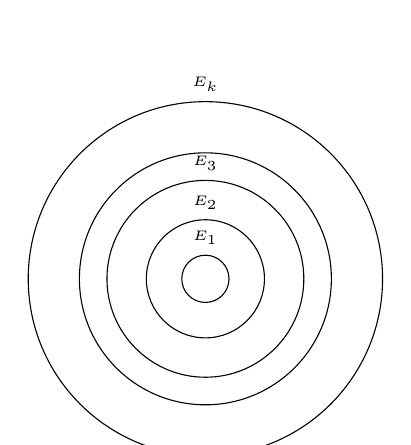
\begin{tikzpicture}
            \node[draw, circle, minimum size =6mm, label=\tiny{$E_1$}] (circle1) at (0,0){};
            \node[draw, circle, minimum size =1.5cm, label=\tiny{$E_2$}] (circle2) at (0,0){};
            \node[draw, circle, thin , minimum size =2.5cm, label=\tiny{$E_3$}] (circle3) at (0,0){};
            \node[draw, circle, thin , minimum size =3.2cm] (circle3) at (0,0){};
            \node[draw, circle, minimum size =4.5cm, label=\tiny{$E_k$}] (circle4) at (0,0){};
        \end{tikzpicture}
    \end{center}
    If $\mu(E_k)=\infty$ for some $k\in\mathds{N}$, then the equitation above is holds because both side equal $\infty$. Hence we can consider only the case where
    $\mu(E_k)<\infty\ \ \forall\ k\in\mathds{N}$.

    For convenience, let $E_0=\emptyset$. Then,
    \[
        \bigcup_{k=1}^{\infty}E_k=\bigcup_{j=1}^{\infty}(E_j\setminus E_{j-1})
    \]
    Where union on the right side is a disjoint union. Thus,

    \begin{align*}
        \mu\left( \bigcup_{k=1}^{\infty}E_k \right) &= \sum_{j=1}^{\infty}\mu(E_j\setminus E_{j-1})\\
                                                    &= \lim_{k\to\infty}\sum_{j=1}^{k}\mu(E_j\setminus E_{j-1})\\
                                                    &= \lim_{k\to\infty}\sum_{j=1}^{k}\left( \mu(E_j)-\mu(E_{j-1}) \right)\\
                                                    &= \lim_{k\to\infty}\mu(E_k).
    \end{align*}
    Hence proved.
\end{proof}

\begin{theorem}[]
    Suppose $(X,\mathcal{A},\mu)$ is a measure space and $E_1\supset E_2\supset\ldots$ is a decreasing sequence of sets in $\mathcal{A}$, with $\mu(E_1)<\infty$. Then
    \[
        \mu\left( \bigcap_{k=1}^{\infty}E_k \right) = \lim_{k\to\infty}\mu(E_k).
    \]
\end{theorem}
\begin{proof}
    By De Morgan's law we have,
    \[
        E_1\setminus \bigcap_{k=1}^{\infty}E_k = \bigcup_{k=1}^{\infty}(E_1\setminus E_k).
    \]
    Now $E_1\setminus E_1,\ E_1\setminus E_2,\ E_1\setminus E_3$ is an increasing sequence of sets in $\mathcal{A}$.
    Thus, by \refeq{increasing},
    \begin{align*}
        \mu\left(E_1\setminus \bigcap_{k=1}^{\infty}E_k\right) &= \lim_{k\to\infty}\mu(E_1\setminus E_k)\\
        \mu\left(E_1\setminus \bigcap_{k=1}^{\infty}E_k\right) &= \lim_{k\to\infty}\left( \mu(E_1)-\mu(E_k) \right) \\
        \mu(E_1)-\mu\left( \bigcap_{k=1}^{\infty}E_k \right) &= \mu(E_1)-\lim_{k\to\infty}\mu(E_k)\\
        \mu\left( \bigcap_{k=1}^{\infty}E_k \right) &= \lim_{k\to\infty}\mu(E_k)
    \end{align*}
\end{proof}
\begin{theorem}[measure of union]
    Suppose $(X,\mathcal{A},\mu)$ is a measure space and $D,E\in\mathcal{A}$, with $\mu(D\cap E)<\infty$. Then
    \[
         \mu(D\cup E)=\mu(D)+\mu(E)-\mu(D\cap E).
    \]
\end{theorem}
\begin{proof}
    We have 
    \[
        D\cup E=(D\setminus (D\cap E))\cup(E\setminus (D\cap E))\cup(D\cap E)
    \]
    where every sets in right side are disjoint so from properties of measure,
    \begin{align*}
        \mu(D\cup E)&=\mu(D\setminus (D\cap E)) + \mu(E\setminus (D\cap E)) + \mu(D\cap E)\\
                    &=\mu(D) - \mu(D\cap E) + \mu(E) - \mu(D\cap E) + \mu(D\cap E)\\
                    &=\mu(D)+\mu(E)-\mu(D\cap E).
    \end{align*}
    Hence proved.
\end{proof}

\section{Lebesgue Measure}

While outer measure has the advantage that it is defined for all sets but we see in \refeq{no length for all set} that it is not additive.
However outer Measure become measure if we suitably reduce the family of sets on which it is defined.
\begin{definition}[Lebesgue Measurable set]
    A set $E$ is said to be  \textit{Lebesgue measurable set} or simply  \textit{measurable set} if for each set $A$ we have 
    \[
        \smu(A)=\smu(A\setminus E^{c})+\smu(A\setminus E)
    \]
\end{definition}

\textbf{Note:} Outer measure is countable subadditive so it always holds $\smu(A)\le \smu(A\setminus E^{c})+\smu(A\setminus E)$ so to proving $E$ is measurable showing 
$\smu(A)\ge \smu(A\setminus E^{c})+\smu(A\setminus E)$ is enough. 

\textbf{Note:} From definition we see that if $E$ is measurable then  $E^{c}$ is also measurable. Clearly $\emptyset$ is a Lebesgue measurable set then $\mathds{R}$ is also measurable.

\begin{theorem}
    \label{measure0}
    If $\smu(E)=0$, then  $E$ is Lebesgue measurable set.
\end{theorem}
\begin{proof}
    Let $A$ is any set. Then  $A\cap E\subset E$, So,
    \[
        \smu(A\cap E)\le \smu(E)=0
    \]
    But $\smu(A\cap E)\ge 0$ so, $\smu(A\cap E)=0$.\\
    Also $A\subset A\cap E^{c}$, then,
    \[
        \smu(A)\ge \smu(A\cap E^{c})=\smu(A\cap E^{c})+\smu(A\cap E)
    \]
    Hence $E$ is Lebesgue measurable set.
\end{proof}

\begin{theorem}[]
    \label{union is measurable}
    If $E_1$ and $E_2$ are Lebesgue measurable set. Then  $E_1\cup E_2$ is Lebesgue measurable.
\end{theorem}
\begin{proof}
    Let $A$ be any set. Since  $E_1$ is measurable,
    \[
        \smu(A)=\smu(A\cap E_1)+\smu(A\cap E_1^{c}).
    \]
    Again $E_2$ is measurable then,
    \[
        \smu(A\cap E_1^{c})=\smu((A\cap E_1^{c})\cap E_2)+\smu((A\cap E_1^{c})\cap E_2^{c})
    \]
    Now, $(A\cap E_1^{c})\cap E_2^{c}=A\cap(E_1^{c}\cap E_2^{c})=A\cap(E_1\cup E_2)^{c}$.
    \\Now,
    \[
        \smu(A)=\smu(A\cap E_1)+\smu(A\cap E_1^{c}\cap E_2)+\smu(A\cap (E_1\cup E_2)^{c})
    \]
    We see, $A\cap(E_1\cup E_2)=(A\cap E_1)\cup(A\cap E_2\cap E_1^{c})$ 
    \\So by property of outer measure, $\smu(A\cap(E_1\cup E_2))\le \smu(A\cap E_1)+\smu(A\cap E_2\cap E_1^{c})$\\
    Then,
    \[
        \smu(A)\ge \smu(A\cap(E_1\cup E_2))+\smu(A\cap (E_1\cup E_2)^{c})
    \]
    Hence, $E_1\cup E_2$ is also Lebesgue measurable.
\end{proof}

\begin{theorem}[]
    \label{sigma-algebra}
    The collection $\mathcal{L}$ of Lebesgue Measurable sets is a \sig-algebra.
\end{theorem}
\begin{proof}
    Let $A$ be any set. \\
    Now,  $A\cap\emptyset=\emptyset$ and $A\cap\emptyset^{c}=A$ So,
    \[
        \smu(A)=\smu(A\cap\emptyset)+\smu(A\cap\emptyset^{c}).
    \]
    Hence, $\emptyset\in\mathcal{L}$ and $X\in\mathcal{L}$ (say, $\emptyset^c=X$).\\
    Now from definition we say if $E\in \mathcal{L}$ then  $E^{c}\in\mathcal{L}$.\\
    Hence, $\mathcal{L}$ is closed under complementation.\\
    Now from \refeq{union is measurable} we say if  $E_1,E_2\in\mathcal{L}$ then  $E_1\cup E_2\in\mathcal{L}$. \\
    Now from previous $E_1^{c},E_2^{c}\in\mathcal{L}$. Then $(E^{c}\cup E^{c})\in\mathcal{L}$.\\
    Then, $(E_1\cap E_2)^{c}\in\mathcal{L}\implies(E_1\cap E_2)\in\mathcal{L}$.\\
    Now using induction on \refeq{union is measurable} we get, $F_n=\cup_{k=1}^{n}E_k\in\mathcal{L}$ where each $E_k\in\mathcal{L}$.\\
    ( 
    if $\{E_n\}$ is sequence of sets in $\mathcal{L}$. Then we can construct another sequence of disjoint sets ${E'_n}$ in  $\mathcal{L}$.
    Where $E'_1=E_1,\ E'_n=E_n\setminus \cup_{k=1}^{n-1}E_k$\\
    and $\cup_{k=1}^{n}E_k=\cup_{k=1}^{n}E'_k$
    )\\
    Without lose of generality we choose $\{E_n\}$ is sequence of disjoint set.\\
    Now $F_n$ is measurable Then,
    \begin{equation}
        \label{Fn measurable}
        \smu(A)=\smu(A\cap F_n)+\smu(A\cap F_n^{c}).
    \end{equation}
    Let, for all $A$ and for some $n\in\mathds{Z}^{+}$ 
    \[
        \smu(A\cap F_n)=\sum_{k=1}^{n}\smu(A\cap E_k).
    \]
    Then, 
    \begin{align*}
        \smu(A\cap F_{n+1})&=\smu((A\cap F_{n+1})\cap F_n)+\smu((A\cap F_{n+1})\cap F_n^{c})\ (\because F_n\ \text{is measurable.})\\
                           &=\smu(A\cap F_n)+\smu(A\cap E_{n+1})\ (\because F_{n+1}\cap F_n^{c}=E_{n+1}).\\
                           &=\sum_{k=1}^{n}\smu(A\cap E_k)+\smu(A\cap E_{n+1})\\
                           &=\sum_{k=1}^{n+1}\smu(A\cap E_k).
    \end{align*}
    Hence the proposition is true for $n+1$. And it is true for  $n=1$.\\
    Hence for all $n$
    \begin{equation}
        \label{FnEn}
        \smu(A\cap F_n)=\sum_{k=1}^{n}\smu(A\cap E_k).
    \end{equation}
    Let, $E=\cup_{k=1}^{n}E_k$. Then clearly $F_n\subset E$ for all $n$.\\
    Then, 
    \begin{align*}
        \smu(A\cap E)&\ge \smu(A\cap F_n) \ \text{ By monotone property}\\
                     &=\sum_{k=1}^{n}\smu(A\cap E_k).
    \end{align*}
    making  $n\to\infty$, We have,
    \begin{align*}
        \smu(A\cap E)\ge \sum_{k=1}^{\infty}\smu(A\cap E_k).
    \end{align*}
    by countable subadditivity, the converse inequality holds. Then,
    \begin{equation}
        \label{infty}
        \smu(A\cap E)=\sum_{k=1}^{\infty}\smu(A\cap E_k)
    \end{equation}
    From \refeq{Fn measurable} and \refeq{FnEn} we have.
    \begin{equation}
        \smu(A)=\sum_{k=1}^{n}\smu(A\cap E_k)+\smu(A\cap F_n^{c})
    \end{equation}
    now clearly $(A\cap F_n^{c})\supset (A\cap E^{c})\implies\smu(A\cap F_n^{c})\ge \smu(A\cap E^{c})$
    Then,
    \begin{equation}
        \label{EnE}
        \smu(A)\ge \sum_{k=1}^{n}\smu(A\cap E_k)+\smu(A\cap E^{c})
    \end{equation}
    Making $n\to\infty$ in \refeq{EnE} We get,
    \begin{align*}
        \smu(A)&\ge \sum_{k=1}^{\infty}\smu(A\cap E_k)+\smu(A\cap E^{c})\\
               &\ge \smu(A\cap E)+\smu(A\cap E^{c}) \ (\text{By \refeq{infty}})
    \end{align*}
    Hence $E=\cup_{k=1}^{\infty}E_k$ is measurable. In other word $\mathcal{L}$ is closed under countable union.\\
    Hence $\mathcal{L}$ is a \sig-algebra.
\end{proof}
Hence outer measure become measure (i.e. additive) when it is restricted on \sig-algebra.
\begin{definition}[Lebesgue Measure]
    Let $\smu$ is outer measure on  $\mathds{R}$ (set of all real number) and $\mathcal{L}$ is a collection of Lebesgue measurable set.
    Then $\smu$ is \textit{Lebesgue Measure} on the measure space $(\mathds{R},\mathcal{L},\smu)$.
\end{definition}

Since Lebesgue Measure is a measure so it follows all the property of measure.

\begin{theorem}
    \label{open mesure}
    The interval $(a,\infty)$ is Lebesgue measurable.
\end{theorem}
\begin{proof}
    To prove $(a,\infty)$ is measurable we show, for any set $A$,
    \begin{align*}
        \smu(A)&=\smu(A\cap(a,\infty))+\smu(A\cap(a,\infty)^{c})\\
        i.e.\ \smu(A)&\ge \smu(A\cap(a,\infty))+\smu(A\cap(-\infty,a]).
    \end{align*}
    Let, $A_1=A\cap(a,\infty)$ and $A_2=A\cap(-\infty,a]$.\\
    If $\smu(A)=\infty$ then we are done.\\
    If $\smu(A)<\infty$, then given $\epsilon>0$ there exist countable collection  $\{I_n\}$ of open intervals which cover  $A$ and for which,
    \[
        \sum_{k=1}^{\infty}\ell(I_k)\le \smu(A)+\epsilon.
    \]
    (Because, $\smu(A)=\inf\left\{ \sum_{k=1}^{\infty}I_k \right\}$ where, $A\subset\cup_{k=1}^{\infty}I_k$ )\\
    Let, $I'_n=I_n\cap(a,\infty)$ and $I''_n=I_n\cap(-\infty,a)$.\\
    Then $I'_n$ and  $I''_n$ are interval(can be empty) and,
    \begin{align*}
        \ell(I_n)&=\ell(I'_n)+\ell(I''_n)\\
                 &=\smu(I'_n)+\smu(I''_n).
    \end{align*}
    Since, $A_1\subset\bigcup_{k=1}^{\infty}I'_k$ we have,
    \[
        \smu(A_1)\le \smu\left( \bigcup_{k=1}^{\infty}I'_k \right) \le \sum_{k=1}^{\infty}\smu(I'_k).
    \]
    Since, $A_2\subset\bigcup_{k=1}^{\infty}I''_k$ we have,
    \[
        \smu(A_2)\le \smu\left( \bigcup_{k=1}^{\infty}I''_k \right) \le \sum_{k=1}^{\infty}\smu(I''_k).
    \]
    Then,
    \begin{align*}
        \smu(A_1)+\smu(A_2)&\le \sum_{k=1}^{\infty}\smu(I'_k)+\sum_{k=1}^{\infty}\smu(I''_k)\\
                           &=\sum_{k=1}^{\infty}\left( \smu(I'_k)+\smu(I''_k) \right)\\
                           &=\sum_{k=1}^{\infty}\ell(I_k)\\
                           &\le \smu(A)+\epsilon.
    \end{align*}
    Since $\epsilon$ is a arbitrary positive real number so we have,
    \[
        \smu(A)\ge \smu(A_1)+\smu(A_2).
    \]
    Hence, $(a,\infty)$ is a measurable set.
\end{proof}

\begin{theorem}[Borel Set are measurable]
    Every Borel set is Lebesgue measurable set.
\end{theorem}
\begin{proof}
    Let $\mathcal{L}$ is a collection of Lebesgue measurable sets. Then by (\refeq{sigma-algebra}) $\mathcal{L}$ is a \sig-algebra and by (\refeq{open mesure})
    $(a,\infty)\in\mathcal{L}$ for all $a\in\mathds{R}$\\
    Then, $(a,\infty)^{c}=(-\infty,a]\in\mathcal{L}$.\\
    Since,
    \[
        (-\infty,b)=\bigcup_{n=1}^{\infty}\left(-\infty,b-\frac{1}{n}\right]
    \]
    then, $(-\infty,b)\in\mathcal{L}$\\
    Again, $(a,b)=(\infty,b)\cap(a,\infty)$. Then, $(a,b)\in\mathcal{L}$.\\
    Now, every open set is union of countable number of open intervals. So, every open set must belong to  $\mathcal{L}$.\\
    Therefor,  $\mathcal{L}$ is a \sig-algebra containing every open set.\\
    Therefor, $\mathcal{L}$ contain the family  $\mathcal{B}$ of Borel Set. As $\mathcal{B}$ is the smallest \sig-algebra containing every open set.\\
    Hence, Borel sets are Lebesgue measurable.
\end{proof}

\begin{theorem}[Alternative Definition of Lebesgue Measure]
    For any set $E\subset\mathds{R}$ the followings are equivalent.
    \begin{enumerate}
        \item $E$ is measurable.
        \item Given  $\epsilon>0$, there is an open set  $O\supset E$ with  $\smu(O\setminus E)<\epsilon$.
        \item Given $\epsilon>0$, there is a closed set  $F\subset E$ with  $\smu(E\setminus F)<\epsilon$.
        \item There exist close sets $F_1,F_2,\ldots$ contained in $E$ such that  $\smu(A\setminus \bigcup_{K=1}^{\infty}F_k)$.
        \item The exist a Borel set $B\subset E$ such That  $\smu(E\setminus B)=0$.
        \item Ther exist open sets $G_1,G_2,\ldots$ containing $E$ such that  $\smu(\bigcap_{k=1}^{\infty}G_k\setminus E)=0$
        \item The exist a Borel set $B\supset E$ such that  $\smu(B\setminus E)=0$.
    \end{enumerate}
\end{theorem}
\begin{proof}
    \textbf{$(1)\implies(2)$}\\
    if $\smu(E)=\infty$ then the result is trivial.
    Let $\smu(E)<\infty$, Then given $\epsilon>0$ there exist countable collection  $\{I_n\}$ of open intervals such that,
     \[
        \sum\ell(I_n)< \smu(E)+\epsilon.
    \]
    Now we know every open set is union of countable open intervals, Then there exist a open set $O$ such that.
    \begin{align*}
        &\smu(O)=\sum\ell(I_n)\\
        i.e.\ &\smu(O)< \smu(E)+\epsilon\\
        i.e.\ &\smu(O)-\smu(E)<\epsilon\\
        i.e.\ &\smu(O\setminus E)<\epsilon\ \ (\because O,E\ \text{both are measurable})
    \end{align*}
    \textbf{$(2)\implies(3)$}\\
    Suppose $(2)$ holds.
    Let $F\subset E$ where  $F$ is close set.\\
    Then,  $E^{c}\subset F^{c}$ here $F^{c}$ is open set.\\
    Then, 
    \begin{align*}
        \smu\left( F^{c}\setminus E^{c} \right)&<\epsilon\\
        \smu\left( E\setminus F \right) &<\epsilon. \ (\because (F^{c}\setminus E^{c})=(E\setminus F)).
    \end{align*}
    \textbf{$(3)\implies(4)$}\\ 
    Suppose $(3)$ holds. Thus for each $n\in\mathds{Z}^{+}$, there exist a close set $F_n\subset E$ such that  $\smu(E\setminus F_n)<\frac{1}{n}$. Now,
    \[
        E\setminus \bigcup_{k=1}^{\infty}F_k\subset E\setminus F_n.
    \]
    Thus, $\smu(E\setminus \bigcup_{k=1}^{\infty}F_k)\le \smu(E\setminus F_n)\le \frac{1}{n}$ for each $n\in\mathds{Z}^{+}$.\\
    Hence, $\smu(E\setminus \bigcup_{k=1}^{\infty})=0$, completing the proof.\\
    \textbf{$(4)\implies(5)$}\\
    Because every countable union of closed sets is Borel set, Hence the result.\\
    \textbf{$(2)\implies(6)$}\\ 
    Suppose $(2)$ holds.\\ Thus for each  $n\in\mathds{Z}^{+}$, there exist an open set $G_n\supset E$ such that  $\smu(G_n\setminus E)<\frac{1}{n}$. Now,
    \[
        \left( \bigcap_{k=1}^{\infty}G_k \right)\setminus A\subset G_n\setminus A. 
    \]
    Thus $\smu\left(\left( \bigcap_{k=1}^{\infty}G_k \right)\setminus A\right)\le \smu\left( G_n\setminus A\right)\le \frac{1}{n}$ for each $n\in\mathds{Z}^{+}$.\\
    Hence $\smu\left( G_n\setminus A\right)=0$, completing the proof.
    \textbf{$(6)\implies(7)$}\\
    Because every countable intersection of open set is a borel set. Hence the result is proved.
    \textbf{$(5)\implies(1)$}\\
    Suppose $(5)$ holds. Thus there exist a borel set  $B\subset E$ such that  $\smu(E\setminus B)=0$.
    Then, $E\setminus B\in \mathcal{L}$ by \refeq{measure0}. Now, 
    \[
        E=B\cup(E\setminus B).
    \]
    Since $B\in\mathcal{L}$,  $(E\setminus B)\in\mathcal{L}$ and  $\mathcal{L}$ is \sig-algebra,  $E\in\mathcal{L}$.\\
    Hence  $E$ is measurable.\\
    \textbf{$(7)\implies(1)$}\\
    Suppose $(7)$ Holds. Thus there exist a borel set  $B\supset E$ such that  $\smu(B\setminus E)=0$
    Now, $B\setminus E$ measurable implies $R\setminus (B\setminus E)$ is also measurable and $B$ is measurable (AS Borel Sets are measurable)
     \[
        E=B\cap(\mathds{R}\setminus (B\setminus E)).
    \]
    Thus, $E$ is also measurable.
\end{proof}

\section{Cantor Set}
Every countable set has outer measure $0$. So the natural question is the converse holds. In other word, is every set with outer measure  $0$ countable?

To construct a cantor set we start with interval $[0,1]$ and removing the middle-third open interval at each step of remaining intervals from previous step.

At first step we remove  $G_1=(\frac{1}{3},\frac{2}{3})$ then we have $[0,1]\setminus G_1=[0,\frac{1}{3}]\cup[\frac{2}{3},1]$.\\
In the second step we remove $G_1\cup G_2=(\frac{1}{3},\frac{2}{3})\cup(\frac{1}{9},\frac{2}{9})\cup(\frac{7}{9},\frac{8}{9})$. Then we left with 
\[
    \left[ 0,1 \right]\setminus (G_1\cup G_2) = \left[0,\frac{1}{9}\right]\cup\left[ \frac{2}{9},\frac{1}{3} \right] \cup \left[ \frac{2}{3},\frac{7}{9} \right] \cup\left[ \frac{8}{9},1\right] 
\]
repeating this presses we construct cantor set.

\begin{definition}[Cantor Set]
    The cantor set $C$ is  $[0,1]\setminus (\bigcup_{k=1}^{\infty}G_k)$, where $G_1=(\frac{1}{3}.\frac{2}{3})$ and $G_n$ for  $n>1$ is the union of the middle-third
    open intervals in the interval of  $[0,1]\setminus (\bigcup_{k=1}^{n-1}G_k$).
\end{definition}
\begin{figure}[!h]
    \centering
    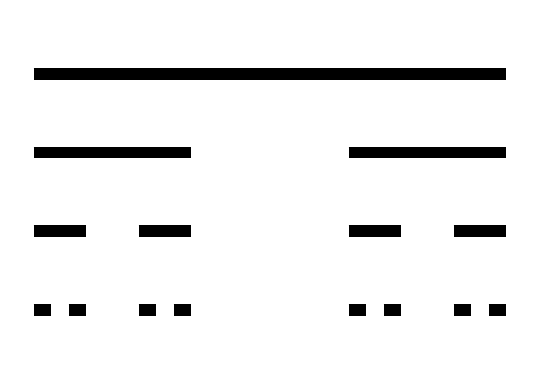
\begin{tikzpicture}[decoration=Cantor set,line width=1.5mm]
        \draw (0,0) -- (6,0);
        \draw decorate{ (0,-1) -- (6,-1) };
        \draw decorate{ decorate{ (0,-2) -- (6,-2) }};
        \draw decorate{ decorate{ decorate{ (0,-3) -- (6,-3) }}};
        \draw decorate{ decorate{ decorate{ decorate{ (0,-4) -- (6,-4) }}}};
    \end{tikzpicture}
    \caption{Cantor Set}
\end{figure}

\begin{theorem}
    \ 
    \begin{enumerate}
        \item The Cantor set is a closed subset of $\mathds{R}$.
        \item The Cantor set has Lebesgue measure $0$.
        \item The Cantor contains no interval with more then one one element.
    \end{enumerate}
\end{theorem}
\begin{proof}
    Each set $G_n$ used in the definition of cantor set is a union of open intervals. Thus  $G_n$ is open. Thus  $\bigcup_{n=1}^{\infty}G_n$ is open set,
    and hence its complement is closed. The Cantor set equals $[0,1]\cap\left( \mathds{R}\setminus \bigcup_{n=1}^{\infty}G_n \right)$, which is the intersection of 
    two closed sets. Thus the Cantor set is a closed, completing the proof of (1).

    By induction on $n$, each  $G_n$ is the union of  $2^{(n-1)}$ disjoint open interval, each of which length  $\frac{1}{3^{n}}$. Thus $\smu(G_n)=\frac{2^{n-1}}{3^{n}}$.
    The set $G_1,G_2,\ldots$ are disjoint. Hence,
    \begin{align*}
        \smu\left( \bigcup_{n=1}^{\infty}G_n \right) &= \frac{1}{3}+\frac{2}{9}+\frac{4}{27}+\ldots\\
                                                     &= \frac{1}{3}\left( 1 +\frac{2}{3}+\frac{4}{9}+\ldots\right) \\
                                                     &=\frac{1}{3}\cdot\frac{1}{1-\frac{2}{3}}\\
                                                     &=1.
    \end{align*}
    Thus the Cantor set, which is equal to $[0,1]\setminus \bigcup_{n=1}^{\infty}G_n$, has Lebesgue measure $1-1$. In other word the Cantor has Lebesgue measure  $0$.
    This proves (2).

    A set with Lebesgue measure  $0$ cannot contain an interval that has more than one element. Thus  $(2)\implies(3)$.
\end{proof}


Now observe that 0 and 1 always belong to  Cantor Set $C$ and all the end points created in each new steps are belong to  the  $C$. 
i.e. $\frac{1}{3},\frac{2}{3}\in C$ and $\frac{1}{9},\frac{2}{9},\frac{7}{9},\frac{8}{9}\in C$, and  $\frac{1}{27},\frac{2}{27},\frac{8}{27},\ldots\in C$.\\
Clearly the numbers which has integer of power 3 in denominator are in $C$. \\
\textbf{\textit{Then  Cantor set is infinite}}.

Now, 0 is always appear in left side of every line segment in all steps. 1 is always appear in right side of every line segment in all steps.
$\frac{1}{3}$ first appear in left line segment and then right in all steps. $\frac{2}{3}$ appear in right ligne segment and then left in all steps.\\
Then we write,
\begin{center}
    \large
    \begin{align*}
        0&= L\ L\ L\ L\ L\ \ldots\\
        1&= R\ R\ R\ R\ R\ \ldots \\
        \frac{1}{3}&= L\ R\ R\ R\ R\ \ldots\\
        \frac{2}{3}&= R\ L\ L\ L\ L\ \ldots\\
        \frac{1}{9}&= L\ L\ R\ R\ R\ \ldots\\
        \frac{2}{9}&= L\ R\ L\ L\ L\ \ldots\\
        \vdots
    \end{align*}
\end{center}
By this way every element of Cantor set can be express in term of infinitely many $L$ and  $R$. In other word every infinite combination of  $L$ and  $R$ 
represent a element of  $C$.

Now, we are changing  $L$ by 0 and  $R$ by 1. Then,
\begin{center}
    \large
    \begin{align*}
        0&= 0\ 0\ 0\ 0\ 0\ \ldots\\
        1&= 1\ 1\ 1\ 1\ 1\ \ldots \\
        \frac{1}{3}&= 0\ 1\ 1\ 1\ 1\ \ldots\\
        \frac{2}{3}&= 1\ 0\ 0\ 0\ 0\ \ldots\\
        \frac{1}{9}&= 0\ 0\ 1\ 1\ 1\ \ldots\\
        \frac{2}{9}&= 0\ 1\ 0\ 0\ 0\ \ldots\\
        \vdots
    \end{align*}
\end{center}
That is ever number of cantor set can be represent by 0's and 1's. 

If possible let us consider, Cantor set is countable. Then we have a countable sequence of number of Cantor set.
Consider,
\begin{center}
    \Large
    \begin{align*}
        & \underbar{0}\ 0\ 0\ 0\ 0\ 0\ 0\ \ldots \\
        & 1\ \underbar{1}\ 1\ 1\ 1\ 1\ 1\ \ldots \\
        & 0\ 1\ \underbar{0}\ 1\ 1\ 0\ 1\ \ldots \\
        & 0\ 1\ 1\ \underbar{1}\ 0\ 1\ 0\ \ldots \\
        & 1\ 1\ 0\ 1\ \underbar{0}\ 0\ 1\ \ldots \\
        & 1\ 0\ 1\ 0\ 1\ \underbar{0}\ 1\ \ldots \\
        & 0\ 0\ 1\ 1\ 0\ 1\ \underbar{0}\ \ldots \\
        &\vdots\ \ \ \ \vdots\ \ \ \ \vdots\ \ \ \ddots 
    \end{align*}
\end{center}
By hypothesis every point of cantor set are in above sequence. But let us consider the number by changing value of $(ii)$(under line position) element in every row.
Then the new number  ($1\ 0\ 1\ 0\ 1\ 1\ 1 \ldots$) is not in above sequence of numbers because it has at least one different digit from ever element in above sequence. But ($1\ 0\ 1\ 0\ 1\ 1\ 1 \ldots$) represent a element of $C$. A contradiction.\\
\textit{\textbf{Cantor Set is uncountable}}.

In fact $C$ contain as many element as  $\mathds{R}$. Although canto set is has measure $0$.

\section{Vitali Set}
We see in \refeq{no length for all set} That every subset of $\mathds{R}$ is not measurable. So, There exist such subset of $\mathds{R}$ which is not measurable.
Vitali set is such nonmeasurable set.

We define a relation on $(0,1]$ by  $x\sim y$ iff  $x-y\in\mathds{Q}$. Then,
\begin{enumerate}
    \item $x\sim x$ as  $x-x=0\in\mathds{Q}$.
    \item if $x\sim y$ then $y\sim x$ as $x-y=y-x\in\mathds{Q}$.
    \item if $x\sim y$ and  $y\sim z$.\\
         Then, $x-y\in\mathds{Q}$ and $y-z\in\mathds{Q}$ \\
         then, $(x-y)+(y-z)=x-z\in\mathds{Q}$ i.e. $x\sim z$.
\end{enumerate}
Hence the above relation is equivalence. Choosing a single point from each equivalence class we construct a set $V$. This construction is possible because of \textit{axiom
of choice} even though it is very controversial topic in mathematics. Without \textit{axiom of choice} it impossible to construct a non measurable set. 
\begin{definition}[Vitali Set]
    A set $V\subset(0,1]$ is called Vitali set if  $V$ contain a single point of  $(x+\mathds{Q})\cap(0,1]$ for each $x+\mathds{Q}\in\mathds{R}/\mathds{Q}$.
\end{definition}
\begin{theorem}
    Vitali set is not Lebesgue measurable.
\end{theorem}
\begin{proof}
    Let $r_1,r_2,\ldots$ be the sequence of all rational number in $[0,1]$. To prove this theory we first proof.
     \begin{enumerate}
         \item if $i\neq j$ then $V+r_i\cap V+r_j=\emptyset$.
         \item $(0,1]=\cup_{i=1}^{\infty}V+r_i$.
    \end{enumerate}
    Where $V+r_i$ is define by  $\{a+x:a\in V\}$ and define 
     $$x+y=
     \begin{cases}
        x+y \ ,\ x+y\le 1 \\
        x+y-1\ ,\ \text{Otherwise}
    \end{cases}
    $$

    \textbf{Proof(1):} Suppose $x\in V+r_i\cap V+r_j$.\\
    Then,  $x=v_i+r_i=v_j+r_j$ for some  $v_i,v_j\in V$ \\
    This implies that $v_i-v_j\in \mathds{Q}$. So,$v_i$ and  $v_j$ belong to same class.\\
    Since  $V$ contain exactly one element of each class. Hence $s_i=s_j$.\\
    Since  $0<r_i,r_j\le 1$ we would also have $r_i=r_j\implies i=j$, completing the prove of (1).

    \textbf{Proof(2):} If  $x\in(0,1]$ then,  $x\sim v$ for some  $v\in V$.\\
    Since  $x$ must be in some equivalence class and representative of each class appears in  $V$.\\ Then $x$ differs from  $y$ by some rational number in  $(0,1]$
    so  $x\in V+r_i$ for some  $i$.\\
    Hence  $(0,1]=\bigcup_{i=1}^{\infty}V+r_i$ proving (2).

    Then we get each $V+r_i$ are disjoint and  $(0,1]=\bigcup_{i=1}^{\infty}V+r_i$.\\
    let $V$ is measurable and  $\smu(V)=a$. Then  $\smu(V+r_i)=a$ as measure is translation invariant.\\
    Then we have, 
    \begin{align*}
        1=\smu((0,1])&=\smu\left( \bigcup_{i=1}^{\infty}V+r_i \right) \\
                     &=\sum_{i=1}^{\infty}\smu(V+r_i)\\
                     &= a+a+a+\ldots 
    \end{align*}
    Now write side is either $0$ or  $\infty$. A contradiction.\\
    Then $V$ is non measurable set.
\end{proof}

\nocite{*}
\bibliographystyle{plain}
\bibliography{refs}

\end{document}
